%% This documentation was generated with Faust version 2.6.3
%% Sun Nov 11 17:05:16 2018
%% https://faust.grame.fr

\documentclass{article}

\usepackage[utf8]{inputenc}
\usepackage{graphicx}
\usepackage[usenames]{color}
\usepackage{listings}
\usepackage{supertabular}
\usepackage{amsmath}
\usepackage{latexsym, amssymb}
\usepackage{breqn}

% No indent
\setlength{\parindent}{0pt}

% Make LaTeX output a dot when typing an asterisk
\DeclareMathSymbol{*}{\mathbin}{symbols}{"01}

% lstlistings setup
\definecolor{yobg}{rgb}{0.9,0.9,1}
\definecolor{yotxt}{rgb}{0.01,0.01,0.52} % a dark blue.
\definecolor{mylstbg}{rgb}{0.98,0.98,0.98} % a really pale grey.
\definecolor{mylstcmt}{rgb}{0.01,0.52,0.01} % a dark green.
\definecolor{mylstdoc}{rgb}{0.80,0.30,0.80} % a medium pink.

\lstset{%
  language=C++, 
  numbers=left,%none,
  tabsize=4, 
  frame=single, 
  breaklines=true, 
  numberstyle=\tiny\ttfamily, 
  backgroundcolor=\color{mylstbg}, 
  basicstyle=\scriptsize\ttfamily, 
  commentstyle=\slshape\color{mylstcmt}, %\itshape,
  frameround=tttt, 
  columns=flexible, %fixed, 
  showstringspaces=false,
  emptylines=2,
  inputencoding=utf8,
  extendedchars=true,
  literate=	{á}{{\'a}}1 
			{à}{{\`a}}1 
			{ä}{{\"a}}1 
			{â}{{\^a}}1
			{é}{{\'e}}1 
			{è}{{\`e}}1 
			{ë}{{\"e}}1 
			{ê}{{\^e}}1
			{ï}{{\"i}}1 
			{î}{{\^i}}1
			{ö}{{\"o}}1 
			{ô}{{\^o}}1
			{è}{{\`e}}1 
			{ù}{{\`u}}1 
			{û}{{\^u}}1
			{ç}{{\c{c}}}1 
			{Ç}{{\c{C}}}1,
  emph={component, declare, environment, import, library, process},
  emph={[2]ffunction, fconstant, fvariable},
  emph={[3]button, checkbox, vslider, hslider, nentry, vgroup, hgroup, tgroup, vbargraph, hbargraph, attach},
  emphstyle=\color{yotxt}, %\underline, %\bfseries,
  morecomment=[s][\color{mylstdoc}]{<mdoc>}{</mdoc>},
  rulecolor=\color{black}
}

\newcommand{\faustfilename}{src/KMHLS\_channel\_map.dsp}
\newcommand{\faustdocdir}{KMHLS\_channel\_map-mdoc}
\newcommand{\faustprogname}{KMHLS\_channel\_map}
\newcommand{\faustversion}{2.6.3}
\newcommand{\faustdocdate}{November 11, 2018}

\begin{document}
\title{KMHLSChannelMap 29+16+4} \author{ Henrik Frisk } \date{\today} \maketitle \begin{tabular}{ll}  \hline  \textbf{author} &  Henrik Frisk  \\  \textbf{copyright} & (c) dinergy 2018  \\  \textbf{filename} & KMHLS\_channel\_map \\  \textbf{license} &  BSD  \\  \textbf{name} & KMHLSChannelMap 29+16+4 \\  \textbf{signals.lib/name} & Faust Signal Routing Library \\  \textbf{signals.lib/version} & 0.0 \\  \textbf{version} &  0.1  \\  \hline \end{tabular} \bigskip  \bigskip This document provides a mathematical description of the Faust program text stored in the \texttt{\faustfilename} file. See the notice in Section\,\ref{notice} (page\,\pageref{notice}) for details.   \section{Mathematical definition of \texttt{process}} \label{equation}  The \emph{\faustprogname} program evaluates the signal transformer denoted by \texttt{process}, which is mathematically defined as follows: 
% Set of Faust formulas (corresponding to an <equation> tag).
\begin{enumerate}

\item Output signals $y_i$ for $i \in [1,52]$ such that
	\begin{dgroup*}
		\begin{dmath*}
				y_{1}(t) = x_{1}(t) * r_{1}(t)
		\end{dmath*}
		\begin{dmath*}
				y_{2}(t) = x_{2}(t) * r_{1}(t)
		\end{dmath*}
		\begin{dmath*}
				y_{3}(t) = x_{3}(t) * r_{1}(t)
		\end{dmath*}
		\begin{dmath*}
				y_{4}(t) = x_{4}(t) * r_{1}(t)
		\end{dmath*}
		\begin{dmath*}
				y_{5}(t) = x_{5}(t) * r_{1}(t)
		\end{dmath*}
		\begin{dmath*}
				y_{6}(t) = x_{6}(t) * r_{1}(t)
		\end{dmath*}
		\begin{dmath*}
				y_{7}(t) = x_{7}(t) * r_{1}(t)
		\end{dmath*}
		\begin{dmath*}
				y_{8}(t) = x_{8}(t) * r_{1}(t)
		\end{dmath*}
		\begin{dmath*}
				y_{9}(t) = x_{9}(t) * r_{1}(t)
		\end{dmath*}
		\begin{dmath*}
				y_{10}(t) = x_{10}(t) * r_{1}(t)
		\end{dmath*}
		\begin{dmath*}
				y_{11}(t) = x_{11}(t) * r_{1}(t)
		\end{dmath*}
		\begin{dmath*}
				y_{12}(t) = x_{12}(t) * r_{1}(t)
		\end{dmath*}
		\begin{dmath*}
				y_{13}(t) = x_{13}(t) * r_{1}(t)
		\end{dmath*}
		\begin{dmath*}
				y_{14}(t) = x_{14}(t) * r_{1}(t)
		\end{dmath*}
		\begin{dmath*}
				y_{15}(t) = x_{15}(t) * r_{1}(t)
		\end{dmath*}
		\begin{dmath*}
				y_{16}(t) = x_{16}(t) * r_{1}(t)
		\end{dmath*}
		\begin{dmath*}
				y_{17}(t) = x_{17}(t) * r_{1}(t)
		\end{dmath*}
		\begin{dmath*}
				y_{18}(t) = x_{18}(t) * r_{1}(t)
		\end{dmath*}
		\begin{dmath*}
				y_{19}(t) = x_{19}(t) * r_{1}(t)
		\end{dmath*}
		\begin{dmath*}
				y_{20}(t) = x_{20}(t) * r_{1}(t)
		\end{dmath*}
		\begin{dmath*}
				y_{21}(t) = x_{21}(t) * r_{1}(t)
		\end{dmath*}
		\begin{dmath*}
				y_{22}(t) = x_{22}(t) * r_{1}(t)
		\end{dmath*}
		\begin{dmath*}
				y_{23}(t) = x_{23}(t) * r_{1}(t)
		\end{dmath*}
		\begin{dmath*}
				y_{24}(t) = x_{24}(t) * r_{1}(t)
		\end{dmath*}
		\begin{dmath*}
				y_{25}(t) = x_{25}(t) * r_{1}(t)
		\end{dmath*}
		\begin{dmath*}
				y_{26}(t) = x_{26}(t) * r_{1}(t)
		\end{dmath*}
		\begin{dmath*}
				y_{27}(t) = x_{27}(t) * r_{1}(t)
		\end{dmath*}
		\begin{dmath*}
				y_{28}(t) = x_{28}(t) * r_{1}(t)
		\end{dmath*}
		\begin{dmath*}
				y_{29}(t) = x_{29}(t) * r_{1}(t)
		\end{dmath*}
		\begin{dmath*}
				y_{30}(t) = 0
		\end{dmath*}
		\begin{dmath*}
				y_{31}(t) = 0
		\end{dmath*}
		\begin{dmath*}
				y_{32}(t) = 0
		\end{dmath*}
		\begin{dmath*}
				y_{33}(t) = x_{30}(t) * r_{2}(t)
		\end{dmath*}
		\begin{dmath*}
				y_{34}(t) = x_{31}(t) * r_{2}(t)
		\end{dmath*}
		\begin{dmath*}
				y_{35}(t) = x_{32}(t) * r_{2}(t)
		\end{dmath*}
		\begin{dmath*}
				y_{36}(t) = x_{33}(t) * r_{2}(t)
		\end{dmath*}
		\begin{dmath*}
				y_{37}(t) = x_{34}(t) * r_{2}(t)
		\end{dmath*}
		\begin{dmath*}
				y_{38}(t) = x_{35}(t) * r_{2}(t)
		\end{dmath*}
		\begin{dmath*}
				y_{39}(t) = x_{36}(t) * r_{2}(t)
		\end{dmath*}
		\begin{dmath*}
				y_{40}(t) = x_{37}(t) * r_{2}(t)
		\end{dmath*}
		\begin{dmath*}
				y_{41}(t) = x_{38}(t) * r_{2}(t)
		\end{dmath*}
		\begin{dmath*}
				y_{42}(t) = x_{39}(t) * r_{2}(t)
		\end{dmath*}
		\begin{dmath*}
				y_{43}(t) = x_{40}(t) * r_{2}(t)
		\end{dmath*}
		\begin{dmath*}
				y_{44}(t) = x_{41}(t) * r_{2}(t)
		\end{dmath*}
		\begin{dmath*}
				y_{45}(t) = x_{42}(t) * r_{2}(t)
		\end{dmath*}
		\begin{dmath*}
				y_{46}(t) = x_{43}(t) * r_{2}(t)
		\end{dmath*}
		\begin{dmath*}
				y_{47}(t) = x_{44}(t) * r_{2}(t)
		\end{dmath*}
		\begin{dmath*}
				y_{48}(t) = x_{45}(t) * r_{2}(t)
		\end{dmath*}
		\begin{dmath*}
				y_{49}(t) = x_{46}(t) * r_{3}(t)
		\end{dmath*}
		\begin{dmath*}
				y_{50}(t) = x_{47}(t) * r_{3}(t)
		\end{dmath*}
		\begin{dmath*}
				y_{51}(t) = x_{48}(t) * r_{3}(t)
		\end{dmath*}
		\begin{dmath*}
				y_{52}(t) = x_{49}(t) * r_{3}(t)
		\end{dmath*}
	\end{dgroup*}

\item Input signals $x_i$ for $i \in [1,49]$ 

\item User-interface input signals  ${u_s}_i$ for $i \in [1,3]$ such that
\begin{itemize}
	\item \textsf{floor ring/}
		\begin{center}
			\begin{supertabular}{lll}
				\textsf{"Volume floor"}  & ${u_s}_{2}(t)$ $\in$ $\left[\,0, 1\,\right]$ & $(\mbox{default value} = 1)$\\
			\end{supertabular}
		\end{center}
	\item \textsf{lower ring/}
		\begin{center}
			\begin{supertabular}{lll}
				\textsf{"Volume dome"}  & ${u_s}_{1}(t)$ $\in$ $\left[\,0, 1\,\right]$ & $(\mbox{default value} = 1)$\\
			\end{supertabular}
		\end{center}
	\item \textsf{subs/}
		\begin{center}
			\begin{supertabular}{lll}
				\textsf{"Volume bass"}  & ${u_s}_{3}(t)$ $\in$ $\left[\,0, 1\,\right]$ & $(\mbox{default value} = 1)$\\
			\end{supertabular}
		\end{center}
	\end{itemize}

\item Intermediate signals  $p_i$ for $i \in [1,3]$ and  $r_i$ for $i \in [1,3]$ such that
	\begin{dgroup*}
		\begin{dmath*}
				p_{1}(t) = 0.001 * {u_s}_{1}(t)
		\end{dmath*}
		\begin{dmath*}
				p_{2}(t) = 0.001 * {u_s}_{2}(t)
		\end{dmath*}
		\begin{dmath*}
				p_{3}(t) = 0.001 * {u_s}_{3}(t)
		\end{dmath*}
	\end{dgroup*}


	\begin{dgroup*}
		\begin{dmath*}
				r_{1}(t) = p_{1}(t) + 0.999 * r_{1}(t\!-\!1)
		\end{dmath*}
		\begin{dmath*}
				r_{2}(t) = p_{2}(t) + 0.999 * r_{2}(t\!-\!1)
		\end{dmath*}
		\begin{dmath*}
				r_{3}(t) = p_{3}(t) + 0.999 * r_{3}(t\!-\!1)
		\end{dmath*}
	\end{dgroup*}

\end{enumerate}

 \section{Block diagram of \texttt{process}} \label{diagram}  The block diagram of \texttt{process} is shown on Figure\,\ref{figure1} (page\,\pageref{figure1}). \begin{figure}[ht!]
	\centering
	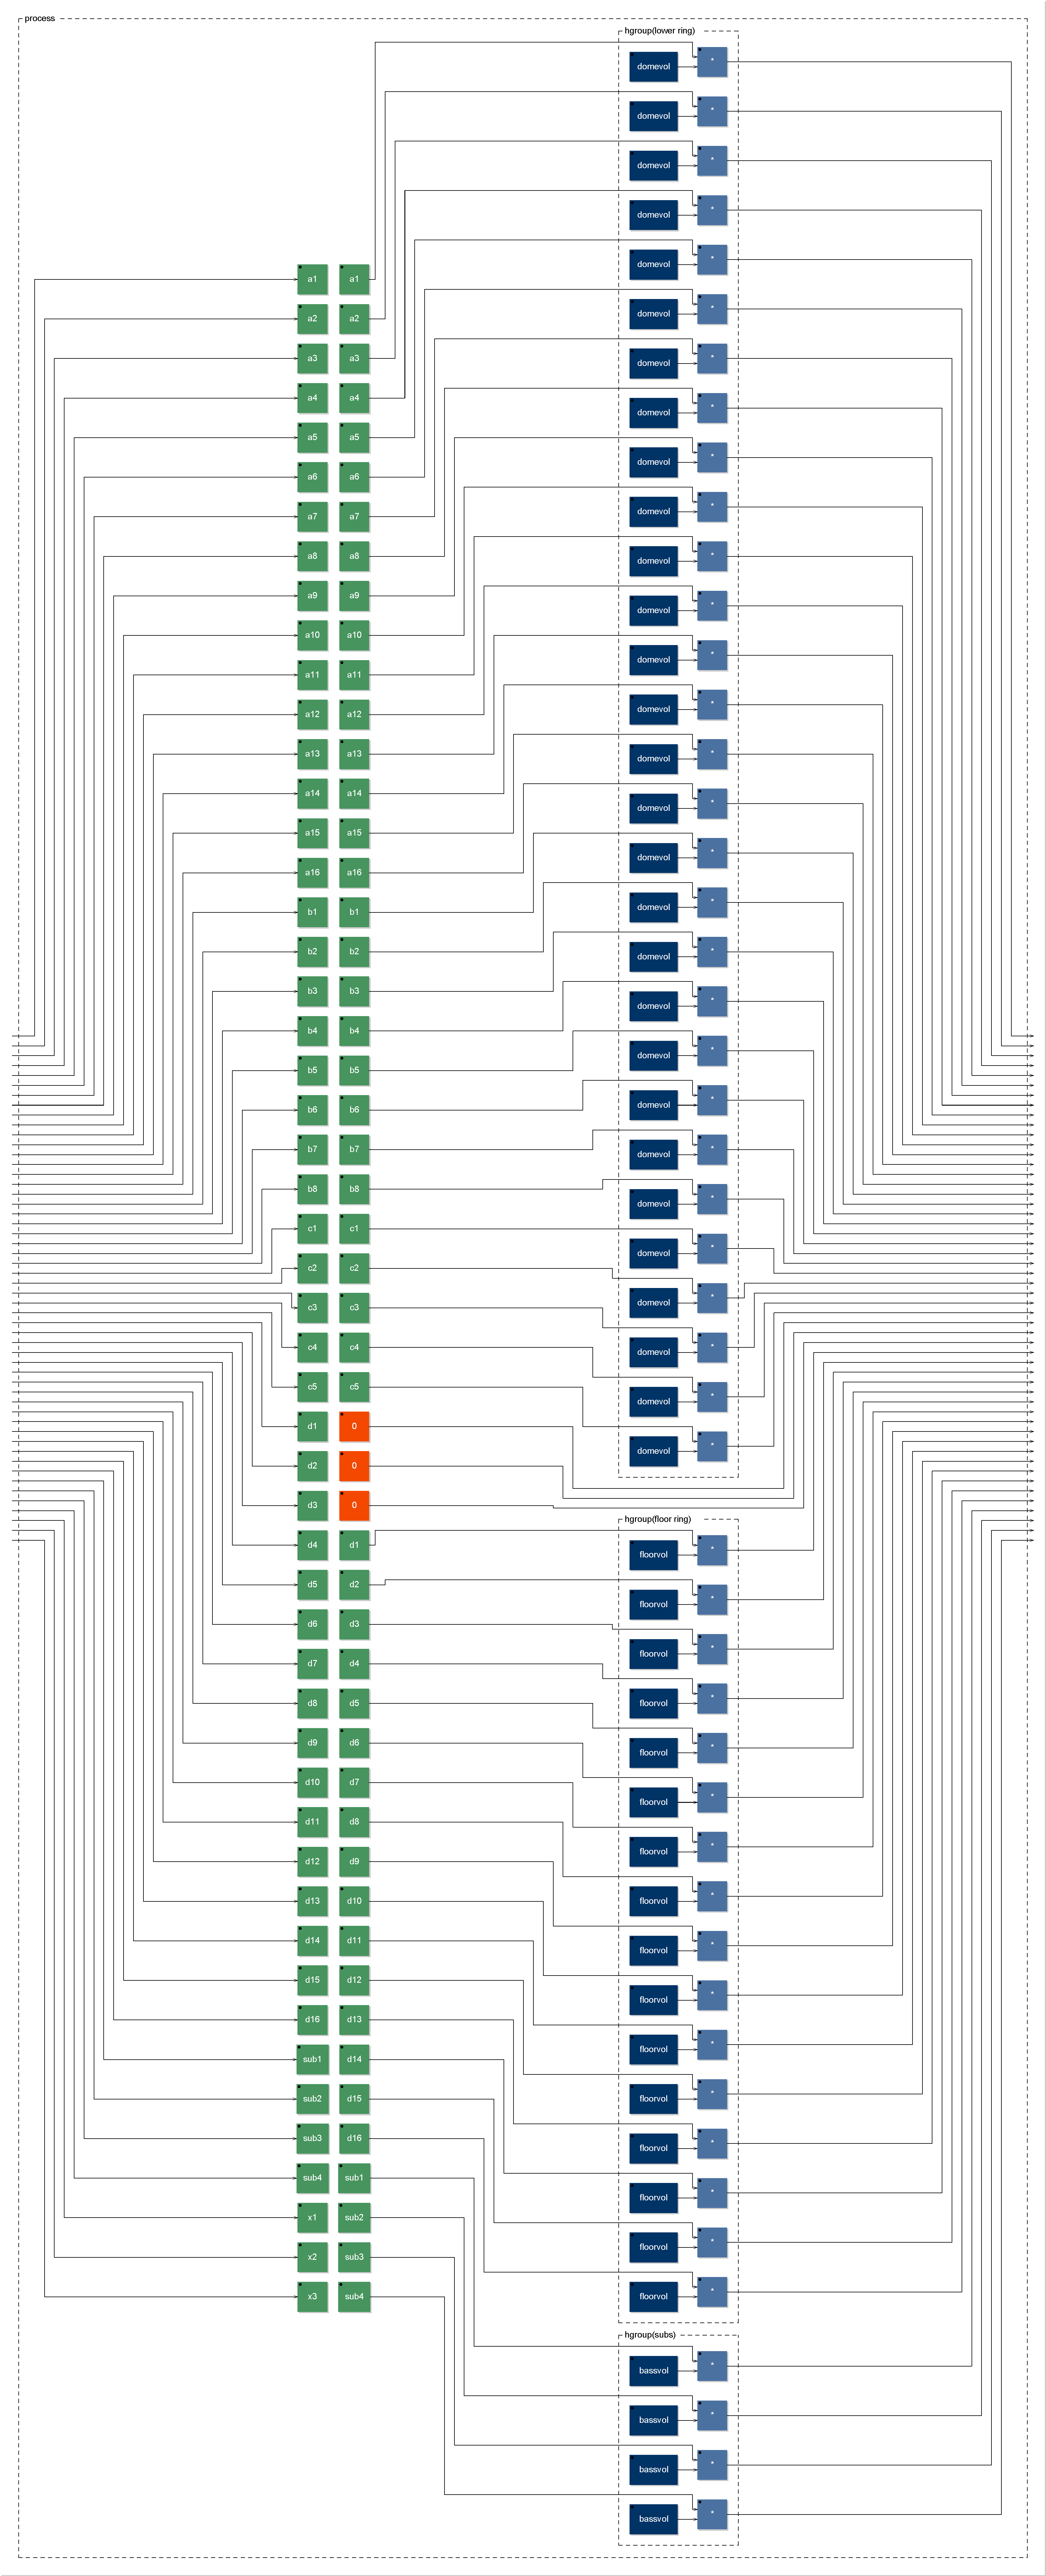
\includegraphics[width=\textwidth]{../svg/svg-01/process}
	\caption{Block diagram of \texttt{process}}
	\label{figure1}
\end{figure}

 \section{Notice} \label{notice}  
\begin{itemize}
	\item This document was generated using Faust version \faustversion\ on \faustdocdate.
	\item The value of a Faust program is the result of applying the signal transformer denoted by the expression to which the \texttt{process} identifier is bound to input signals, running at the $f_S$ sampling frequency.
	\item Faust (\emph{Functional Audio Stream}) is a functional programming language designed for synchronous real-time signal processing and synthesis applications. A Faust program is a set of bindings of identifiers to expressions that denote signal transformers. A signal $s$ in $S$ is a function mapping\footnote{Faust assumes that $\forall \, s \in S, \forall \, t \in \mathbb{Z}, s(t) = 0 \mathrm{\ when\ } t < 0$.} times $t \in \mathbb{Z}$ to values $s(t) \in \mathbb{R}$, while a signal transformer is a function from $S^n$ to $S^m$, where $n,m\in \mathbb{N}$. See the Faust manual for additional information (\textsf{http://faust.grame.fr}).
	\item Every mathematical formula derived from a Faust expression is assumed, in this document, to having been normalized (in an implementation-depen\-dent manner) by the Faust compiler.
	\item A block diagram is a graphical representation of the Faust binding of an identifier I to an expression E; each graph is put in a box labeled by I. Subexpressions of E are recursively displayed as long as the whole picture fits in one page.
	\item The \texttt{\faustdocdir/} directory may also include the following subdirectories:
\begin{itemize}
	\item	\texttt{cpp/} for Faust compiled code; 
	\item	\texttt{pdf/} which contains this document; 
	\item	\texttt{src/} for all Faust sources used (even libraries); 
	\item	\texttt{svg/} for block diagrams, encoded using the Scalable Vector Graphics format (\textsf{http://www.w3.org/Graphics/SVG/});
	\item	\texttt{tex/} for the \LaTeX\ source of this document.
\end{itemize}
\end{itemize}

 \section{Faust code listings} \label{listing}  This section provides the listings of the Faust code used to generate this document, including dependencies. 
\bigskip\bigskip
\begin{lstlisting}[caption=\texttt{KMHLS\_channel\_map.dsp}]
declare name	"KMHLSChannelMap 29+16+4";
declare version " 0.1 ";
declare author " Henrik Frisk " ;
declare license " BSD ";
declare copyright "(c) dinergy 2018 ";

//---------------`Channel mapping plugin` --------------------------
//
// Channel mapping plugin that takes 52 inputs, although only the 49 first channels are routed.
// these are routed to the Crescendo mixer channel layout.
// 
// Insert this plugin on the master track or similar to get channels to map correctly to the Crescendo, i.e.:
// 
// * Channel 1-29 of the input maps to Crescendo 1-29 (Layer A)
// * Channel 30-45 of the input maps to Crescendo 33-48 (Layer B)
// * Channel 46-49 maps to Crescendo 49-52 (Layer B)
//---------------------------------------------------

import("stdfaust.lib");

domevol = hslider("Volume dome", 1., 0., 1., 0.001) : si.smoo;
floorvol = hslider("Volume floor", 1., 0., 1., 0.001) : si.smoo;
bassvol = hslider("Volume bass", 1., 0., 1., 0.001) : si.smoo;

process ( a1, a2, a3, a4, a5, a6, a7, a8, a9, a10, a11, a12, a13, a14, a15, a16,
	 b1, b2, b3, b4, b5, b6, b7, b8,
	 c1, c2, c3, c4, c5,
	 d1, d2, d3, d4, d5, d6, d7, d8, d9, d10, d11, d12, d13, d14, d15, d16,
	 sub1, sub2, sub3, sub4, x1, x2, x3) = a1, a2, a3, a4, a5, a6, a7, a8, a9, a10, a11, a12, a13, a14, a15, a16,
				   b1, b2, b3, b4, b5, b6, b7, b8,
				   c1, c2, c3, c4, c5, 0, 0, 0,
				   d1, d2, d3, d4, d5, d6, d7, d8, d9, d10, d11, d12, d13, d14, d15, d16,
				   sub1, sub2, sub3, sub4
						     : hgroup("lower ring", par(i, 29, _ * domevol)), _, _, _,
				   hgroup("floor ring", par(i, 16, _ * floorvol)),
				   hgroup("subs", par(i, 4, _ * bassvol));
  
\end{lstlisting}


\bigskip\bigskip
\begin{lstlisting}[caption=\texttt{stdfaust.lib}]
//################################ stdfaust.lib ##########################################
// The purpose of this library is to give access to all the Faust standard libraries
// through a series of environment.
//########################################################################################

an = library("analyzers.lib");
ba = library("basics.lib");
co = library("compressors.lib");
de = library("delays.lib");
dm = library("demos.lib");
dx = library("dx7.lib");
en = library("envelopes.lib");
fi = library("filters.lib");
ho = library("hoa.lib");
ma = library("maths.lib");
ef = library("misceffects.lib");
os = library("oscillators.lib");
no = library("noises.lib");
pf = library("phaflangers.lib");
pm = library("physmodels.lib");
re = library("reverbs.lib");
ro = library("routes.lib");
sp = library("spats.lib");
si = library("signals.lib");
so = library("soundfiles.lib");
sy = library("synths.lib");
ve = library("vaeffects.lib");
sf = library("all.lib");
\end{lstlisting}


\bigskip\bigskip
\begin{lstlisting}[caption=\texttt{signals.lib}]
//#################################### signals.lib ########################################
// A library of basic elements to handle signals in Faust. Its official prefix is `si`.
//########################################################################################

/************************************************************************
************************************************************************
FAUST library file, GRAME section

Except where noted otherwise, Copyright (C) 2003-2017 by GRAME,
Centre National de Creation Musicale.

----------------------------------------------------------------------
GRAME LICENSE

This program is free software; you can redistribute it and/or modify
it under the terms of the GNU Lesser General Public License as
published by the Free Software Foundation; either version 2.1 of the
License, or (at your option) any later version.

This program is distributed in the hope that it will be useful,
but WITHOUT ANY WARRANTY; without even the implied warranty of
MERCHANTABILITY or FITNESS FOR A PARTICULAR PURPOSE.  See the
GNU Lesser General Public License for more details.

You should have received a copy of the GNU Lesser General Public
License along with the GNU C Library; if not, write to the Free
Software Foundation, Inc., 59 Temple Place, Suite 330, Boston, MA
02111-1307 USA.

EXCEPTION TO THE LGPL LICENSE : As a special exception, you may create a
larger FAUST program which directly or indirectly imports this library
file and still distribute the compiled code generated by the FAUST
compiler, or a modified version of this compiled code, under your own
copyright and license. This EXCEPTION TO THE LGPL LICENSE explicitly
grants you the right to freely choose the license for the resulting
compiled code. In particular the resulting compiled code has no obligation
to be LGPL or GPL. For example you are free to choose a commercial or
closed source license or any other license if you decide so.
************************************************************************
************************************************************************/

ba = library("basics.lib");
ro = library("routes.lib");
si = library("signals.lib");

declare name "Faust Signal Routing Library";
declare version "0.0";

//=============================Functions Reference========================================
//========================================================================================

//--------------------------------`(si.)bus`-------------------------------------
// n parallel cables.
// `bus` is a standard Faust function.
//
// #### Usage
//
// ```
// bus(n)
// bus(4) : _,_,_,_
// ```
//
// Where:
//
// * `n`: is an integer known at compile time that indicates the number of parallel cables.
//-----------------------------------------------------------------------------
bus(2) = _,_; // avoids a lot of "bus(1)" labels in block diagrams
bus(n) = par(i, n, _);


//--------------`(si.)block`--------------
// Block - terminate n signals.
// `block` is a standard Faust function.
//
// #### Usage
//
// ```
// _,_,... : block(n) : _,...
// ```
//
// Where:
//
// * `n`: the number of signals to be blocked
//--------------------------------------
block(n) = par(i,n,!);


//-----------------------------`(si.)interpolate`-------------------------------
// Linear interpolation between two signals.
//
// #### Usage
//
// ```
// _,_ : interpolate(i) : _
// ```
//
// Where:
//
// * `i`: interpolation control between 0 and 1 (0: first input; 1: second input)
//-----------------------------------------------------------------------------
interpolate(i) = *(1.0-i),*(i) : +;

//------------------------`(si.)smoo`---------------------------------------
// Smoothing function based on `smooth` ideal to smooth UI signals
// (sliders, etc.) down.
// `smoo` is a standard Faust function.
//
// #### Usage
//
// ```
// hslider(...) : smoo;
// ```
//---------------------------------------------------------------------
smoo = si.smooth(0.999);


//-----------------------`(si.)polySmooth`--------------------------------
// A smoothing function based on `smooth` that doesn't smooth when a
// trigger signal is given. This is very useful when making
// polyphonic synthesizer to make sure that the value of the parameter
// is the right one when the note is started.
//
// #### Usage
//
// ```
// hslider(...) : polysmooth(g,s,d) : _
// ```
//
// Where:
//
// * `g`: the gate/trigger signal used when making polyphonic synths
// * `s`: the smoothness (see `smooth`)
// * `d`: the number of samples to wait before the signal start being
// 		smoothed after `g` switched to 1
//-------------------------------------------------------------------
polySmooth(g,s,d) = smooth(s*((g==(g@d)) | (g == 0)));

//-----------------------`(si.)smoothAndH`--------------------------------
// A smoothing function based on `smooth` that holds its output
// signal when a trigger is sent to it. This feature is convenient
// when implementing polyphonic instruments to prevent some
// smoothed parameter to change when a note-off event is sent.
//
// #### Usage
//
// ```
// hslider(...) : smoothAndH(g,s) : _
// ```
//
// Where:
//
// * `g`: the hold signal (0 for hold, 1 for bypass)
// * `s`: the smoothness (see `smooth`)
//-------------------------------------------------------------------
smoothAndH(t,s) = smooth(s*t) : ba.sAndH(t);

//-----------------------------`(si.)bsmooth`------------------------------
// Block smooth linear interpolation during a block of samples.
//
// #### Usage
//
// ```
// hslider(...) : bsmooth : _
// ```
//-----------------------------------------------------------------------
bsmooth(c) = +(i) ~ _
with {
	i = (c-c@n)/n;
	n = min(4096, max(1, fvariable(int count, <math.h>)));
};

//-------------------------------`(si.)dot`--------------------------------------
// Dot product for two vectors of size n.
//
// #### Usage
//
// ```
// _,_,_,_,_,_ : dot(n) : _
// ```
//
// Where:
//
// * `n`: size of the vectors (int, must be known at compile time)
//-----------------------------------------------------------------------------
dot(n) = ro.interleave(n,2) : par(i,n,*) :> _;

// end GRAME section
//########################################################################################
/************************************************************************
FAUST library file, jos section

Except where noted otherwise, The Faust functions below in this
section are Copyright (C) 2003-2017 by Julius O. Smith III <jos@ccrma.stanford.edu>
([jos](http://ccrma.stanford.edu/~jos/)), and released under the
(MIT-style) [STK-4.3](#stk-4.3-license) license.

All MarkDown comments in this section are Copyright 2016-2017 by Romain
Michon and Julius O. Smith III, and are released under the
[CCA4I](https://creativecommons.org/licenses/by/4.0/) license (TODO: if/when Romain agrees!)

************************************************************************/
//-------------------`(si.)smooth`-----------------------------------
// Exponential smoothing by a unity-dc-gain one-pole lowpass.
// `smooth` is a standard Faust function.
//
// #### Usage:
//
// ```
// _ : smooth(tau2pole(tau)) : _
// ```
//
// Where:
//
// * `tau`: desired smoothing time constant in seconds, or
//
// ```
// hslider(...) : smooth(s) : _
// ```
//
// Where:
//
// * `s`: smoothness between 0 and 1. s=0 for no smoothing, s=0.999 is "very smooth",
// s>1 is unstable, and s=1 yields the zero signal for all inputs.
// The exponential time-constant is approximately 1/(1-s) samples, when s is close to
// (but less than) 1.
//
// #### Reference:
//
// <https://ccrma.stanford.edu/~jos/mdft/Convolution_Example_2_ADSR.html>
//-------------------------------------------------------------
smooth(s) = *(1.0 - s) : + ~ *(s);

//--------------------------------`(si.)cbus`-------------------------------------
// n parallel cables for complex signals.
// `cbus` is a standard Faust function.
//
// #### Usage
//
// ```
// cbus(n)
// cbus(4) : (r0,i0), (r1,i1), (r2,i2), (r3,i3)
// ```
//
// Where:
//
// * `n`: is an integer known at compile time that indicates the number of parallel cables.
// * each complex number is represented by two real signals as (real,imag)
//-----------------------------------------------------------------------------
cbus(1) = (_,_);
cbus(n) = par(i, n, (_,_));

//--------------------------------`(si.)cmul`-------------------------------------
// multiply two complex signals pointwise.
// `cmul` is a standard Faust function.
//
// #### Usage
//
// ```
// (r1,i1) : cmul(r2,i2) : (_,_);
// ```
//
// Where:
//
// * Each complex number is represented by two real signals as (real,imag), so
// - `(r1,i1)` = real and imaginary parts of signal 1
// - `(r2,i2)` = real and imaginary parts of signal 2
//-----------------------------------------------------------------------------
cmul(r1,i1,r2,i2) = (r1*r2 - i1*i2), (r1*i2 + r2*i1);

// end jos section
/************************************************************************
FAUST library file, further contributions section
All contributions below should indicate both the contributor and terms
of license.  If no such indication is found, "git blame" will say who
last edited each line, and that person can be emailed to inquire about
license disposition, if their license choice is not already indicated
elsewhere among the libraries.  It is expected that all software will be
released under LGPL, STK-4.3, MIT, BSD, or a similar FOSS license.
************************************************************************/

//-------------`(si.)lag_ud`---------------
// Lag filter with separate times for up and down.
//
// #### Usage
//
// ```
// _ : lag_ud(up, dn, signal) : _;
// ```
//----------------------------------------------------
// Author: Jonatan Liljedahl
// License: STK-4.3
// MarkDown: Romain Michon
lag_ud(up,dn) = _ <: ((>,ba.tau2pole(up),ba.tau2pole(dn):select2),_:si.smooth) ~ _;

// end further further contributions section
\end{lstlisting}


\end{document}

